\section{El modelo}

El modelo encadena cinco partes (figura~\ref{fig:marco}). Cada una entrega a la siguiente un
número con el que se puede diseñar, y todas quedan acotadas por la capa ética y normativa de
la sección~\ref{sec:etica}.

\begin{figure}[H]
\centering
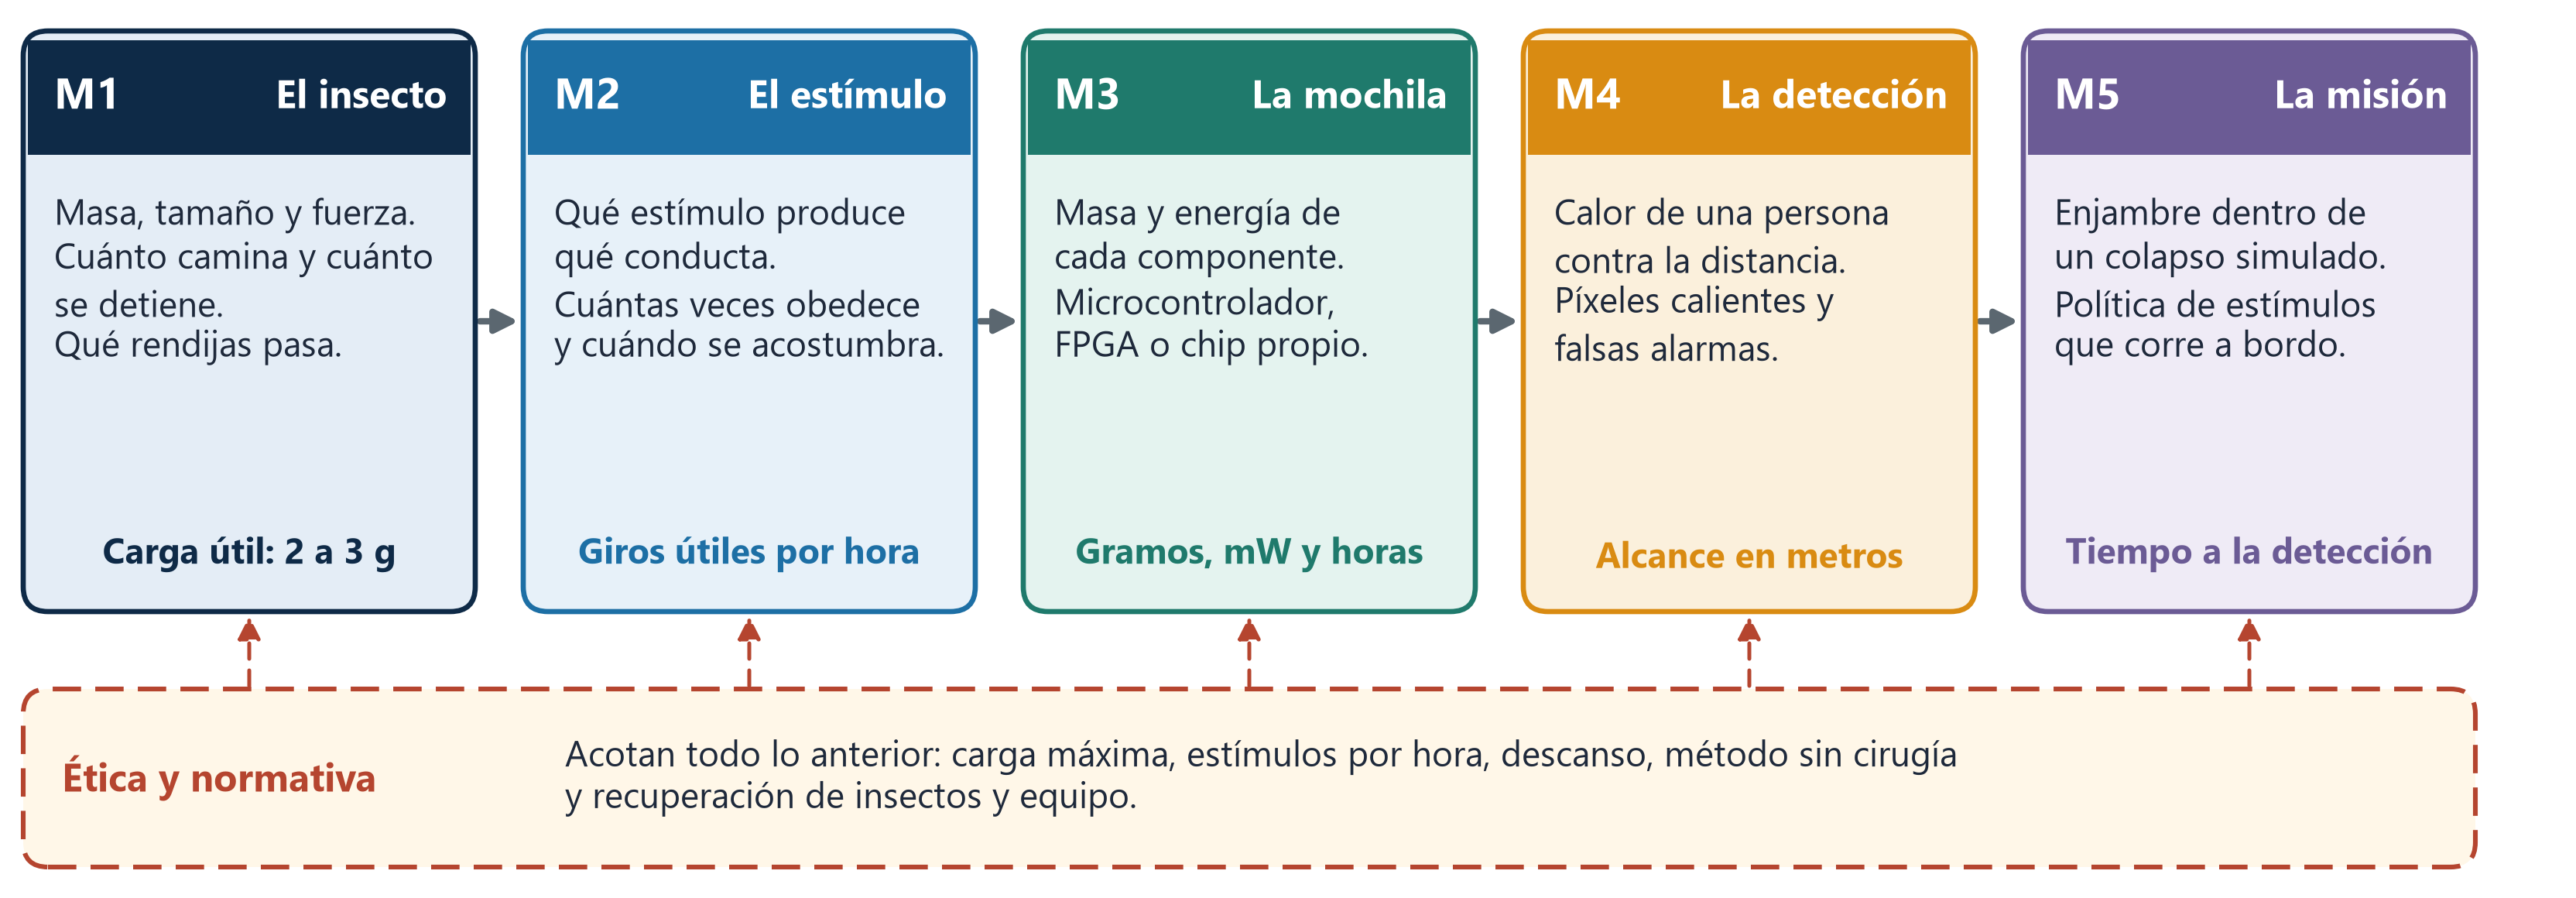
\includegraphics[width=\textwidth]{figs/marco_modelo.png}
\caption{Marco del modelo: cinco submodelos encadenados y la capa que los acota.}
\label{fig:marco}
\end{figure}

\subsection{M1. El insecto: marcha natural}

La marcha sin estímulo se describe con el modelo de Dirafzoon et al.~\cite{dirafzoon2017}, con
los valores que usan Tran-Ngoc et al.~\cite{tranngoc2024}. El insecto camina tramos rectos de
longitud exponencial con media $l^*=17.6$~cm a $v=1.94$~cm/s. Al terminar cada tramo se
detiene con probabilidad $P_s=0.211$ durante un tiempo de media $T_s=36.8$~s; si no se detiene,
gira un ángulo pequeño. Cuando toca una pared la sigue, y solo la suelta con probabilidad
$p_e=0.005$ por tramo. De ahí sale la fracción del tiempo que pasa caminando:
\begin{equation}
F_m=\frac{l^*/v}{l^*/v+P_s\,T_s}=\frac{9.1}{9.1+7.8}=0.54 ,
\end{equation}
dentro del intervalo medido de $0.37\pm0.20$. La carga útil y la altura salen de la
tabla~\ref{tab:capacidades}: $m_c\le3$~g y componentes no apilados.

\subsection{M2. El estímulo}

\begin{table}[H]
\centering\footnotesize
\caption{Tipos de estímulo para dirigir a \Gp.}
\label{tab:estimulos}
\rowcolors{2}{SoftGray}{white}
\begin{tabularx}{\textwidth}{@{}>{\bfseries\raggedright\arraybackslash}p{2.7cm} >{\raggedright\arraybackslash}p{1.5cm} >{\raggedright\arraybackslash}p{3.0cm} >{\raggedright\arraybackslash}p{3.3cm} >{\raggedright\arraybackslash}X@{}}
\toprule
\rowcolor{TableHead} Estímulo & Cirugía & Conducta & Eficacia publicada & Inconveniente \\
\midrule
Electrodo implantado en la antena~\cite{latif2012,erickson2015} & Sí & Giro al lado contrario & 56~\% de los individuos; giros con mediana de 130\textdegree & Inutiliza la antena; el implante dura días \\
Electrodo implantado en los cercos~\cite{tranngoc2023} & Sí & Avance; giro con un solo cerco & 94~\% de navegaciones & Las fuentes no coinciden en el sentido del giro \\
Electrodo torácico~\cite{lin2025} & Poca & Giro y freno & Giro de más de 70\textdegree{} en 0.4~s & Requiere ensamble preciso \\
Electrodo de superficie en antena y abdomen~\cite{lin2023,tranngoc2025} & No & Giro y avance & 81~\% y 74~\% por estímulo; giro medio de 38\textdegree & Impedancia alta: 70 a 123~k$\Omega$ \\
Luz ultravioleta junto a los ojos~\cite{refat2025,gracidas2026} & No & Giro al lado contrario; reanuda la marcha & Sin habituación en 150 ensayos; aumenta la locomoción & Falta medir el ángulo por pulso \\
Calor en los tarsos & No & Escape & Cualitativa & Unos 330~mW por estímulo~\cite{erickson2015}: 100 veces el eléctrico \\
\bottomrule
\end{tabularx}
\end{table}

Todos los estímulos eléctricos usan una onda cuadrada bifásica de 40 a 55~Hz, con ciclo de
trabajo de 50~\% y trenes de 0.4 a 1~s; con electrodo implantado bastan 2 a 3~V, y subir el
voltaje empeora la respuesta~\cite{erickson2015,lin2025}. El tren cuesta unos 2.2~mW mientras
dura~\cite{erickson2015}, así que el estímulo no pesa en la energía.

\textbf{Elección.} Se adopta la luz ultravioleta como estímulo principal, porque no requiere
cirugía, no se ha observado habituación y la misma colonia de la universidad responde a
ella~\cite{gracidas2026}; los electrodos de superficie quedan como alternativa. El generador
de pulsos del núcleo sirve para los dos casos.

\textbf{Respuesta y habituación.} El insecto obedece un estímulo con probabilidad
$p\,(1-H)$, donde $p=0.78$~\cite{lin2023} y $H$ es la habituación. Cada estímulo la sube y el
descanso la baja:
\begin{equation}
H\leftarrow H+\alpha\,(1-H) \quad\text{por estímulo},\qquad
H(t+\Delta t)=H(t)\,e^{-\Delta t/\tau}.
\end{equation}
Con $\tau=600$~s (las fuentes dan de 5 a 20~min de recuperación~\cite{sanchez2015}) y
$\alpha=0.09$, el modelo reproduce los tres datos disponibles para pulsos unipolares: queda el
46~\% de la respuesta tras diez estímulos cada 15~s (medido: 43~\%~\cite{ma2023}), el 71~\% cada
120~s (medido: 66~\%) y el 22~\% tras cuarenta ensayos (medido: 20~\%~\cite{erickson2015}). Con
onda bifásica o con luz, $\alpha$ es al menos cuarenta veces menor (figura~\ref{fig:habituacion}).
La simulación usa $\alpha=0.01$, un valor conservador.

\begin{figure}[H]
\centering
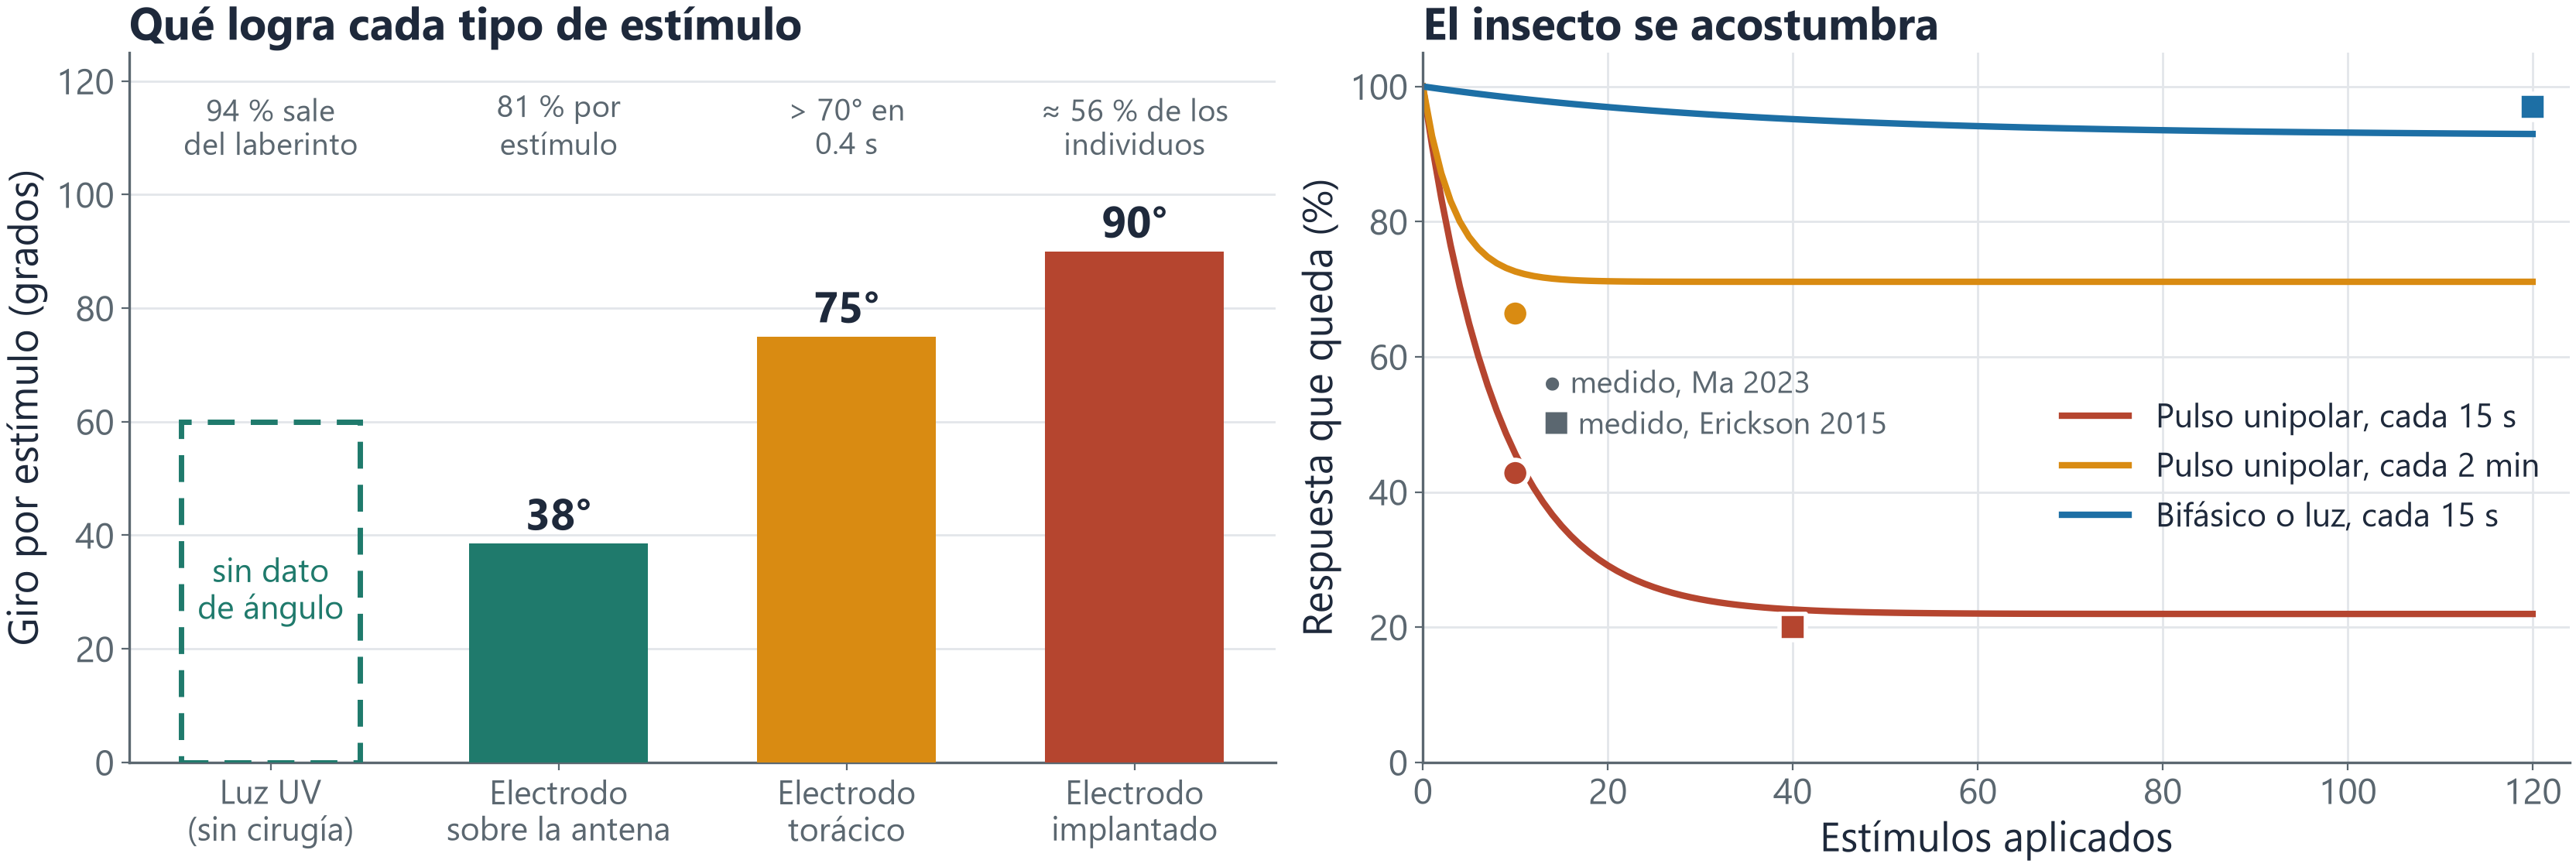
\includegraphics[width=\textwidth]{figs/habituacion.png}
\caption{Izquierda: giro por estímulo según el método~\cite{lin2023,lin2025,ma2023}. Derecha: modelo de
habituación frente a los datos medidos.}
\label{fig:habituacion}
\end{figure}

\subsection{M3. La mochila: masa, energía y cómputo}

\begin{figure}[H]
\centering
\begin{subfigure}{0.49\textwidth}
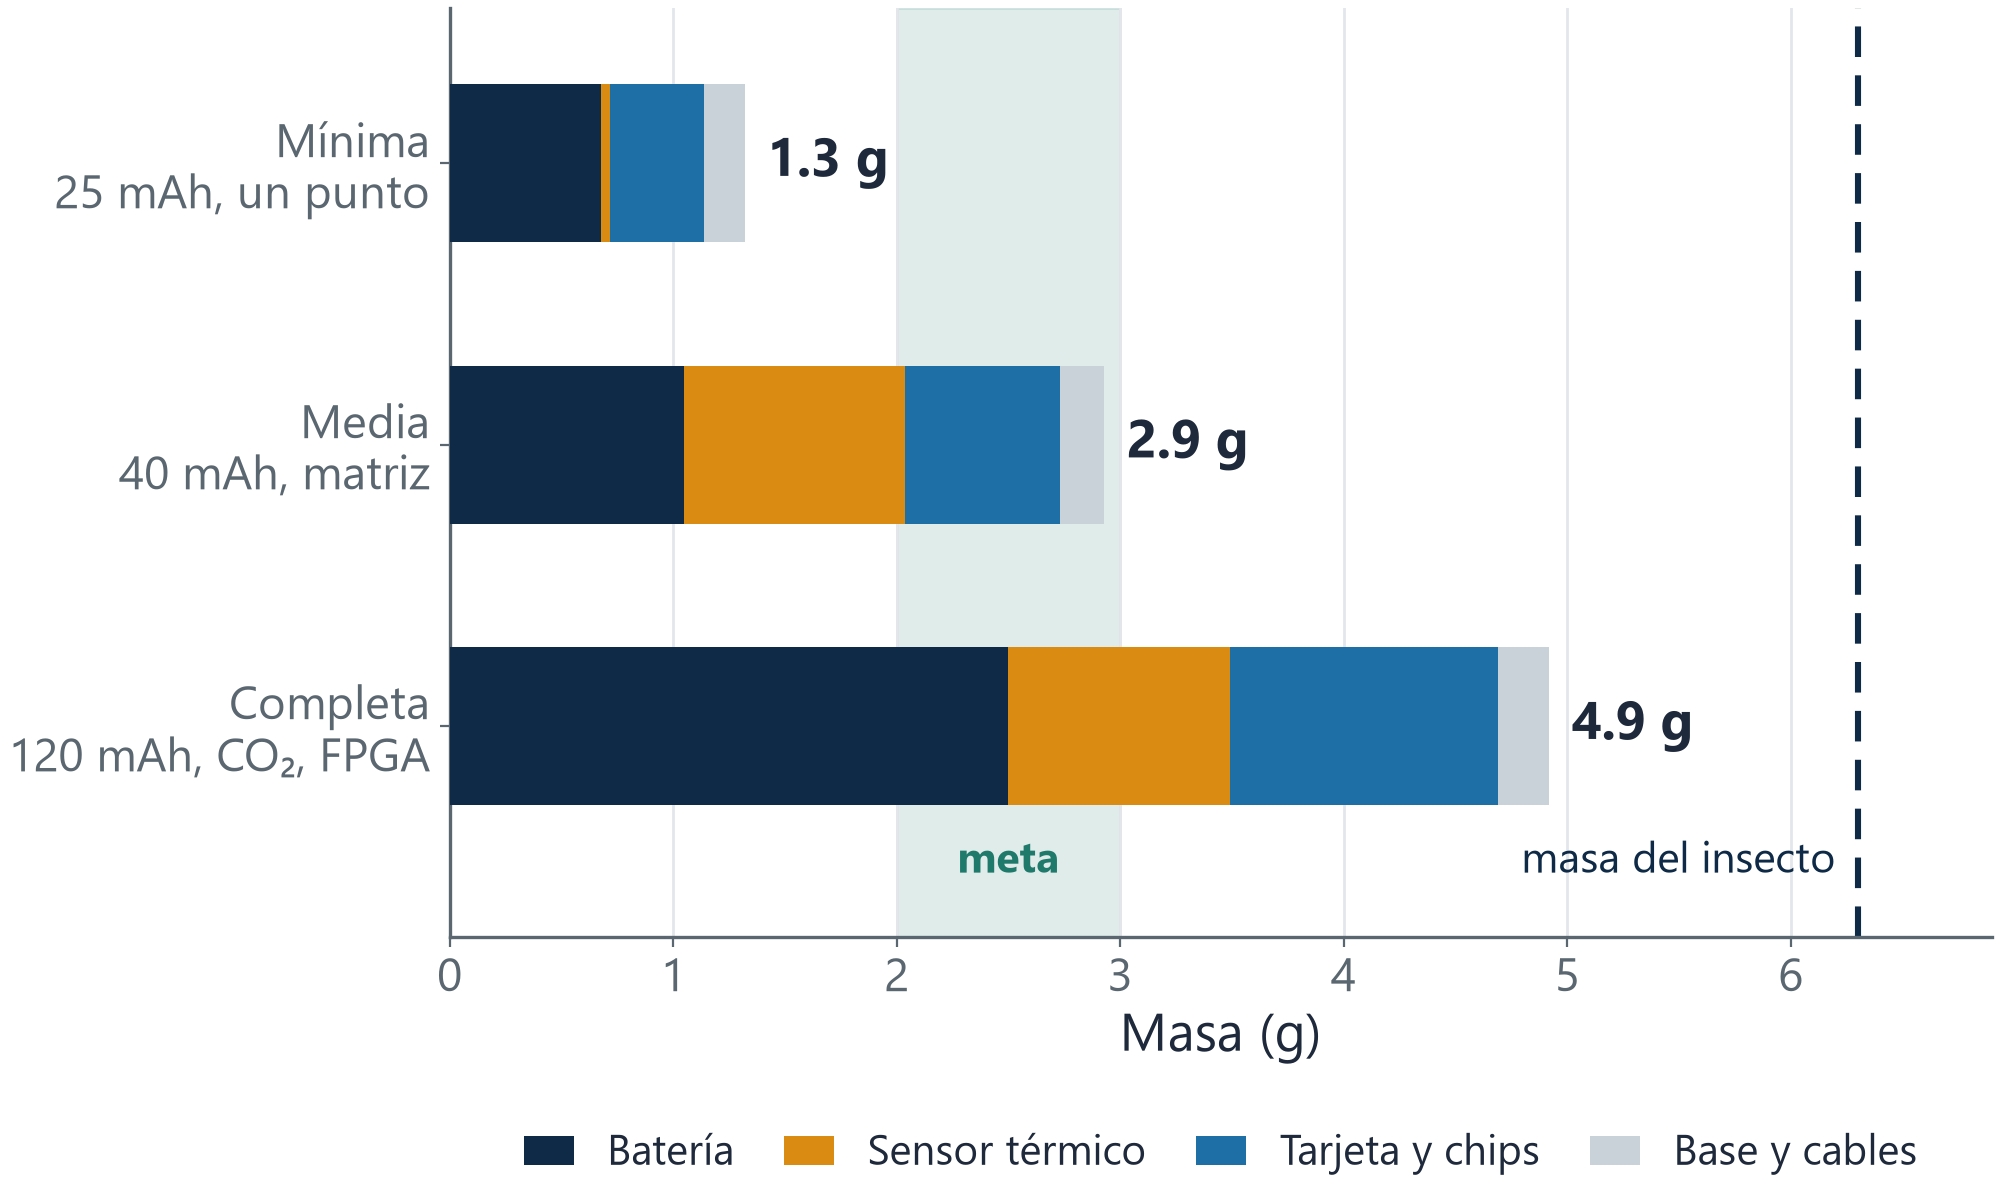
\includegraphics[width=\linewidth]{figs/presupuesto_masa.png}
\caption{Masa por configuración.}
\end{subfigure}\hfill
\begin{subfigure}{0.49\textwidth}
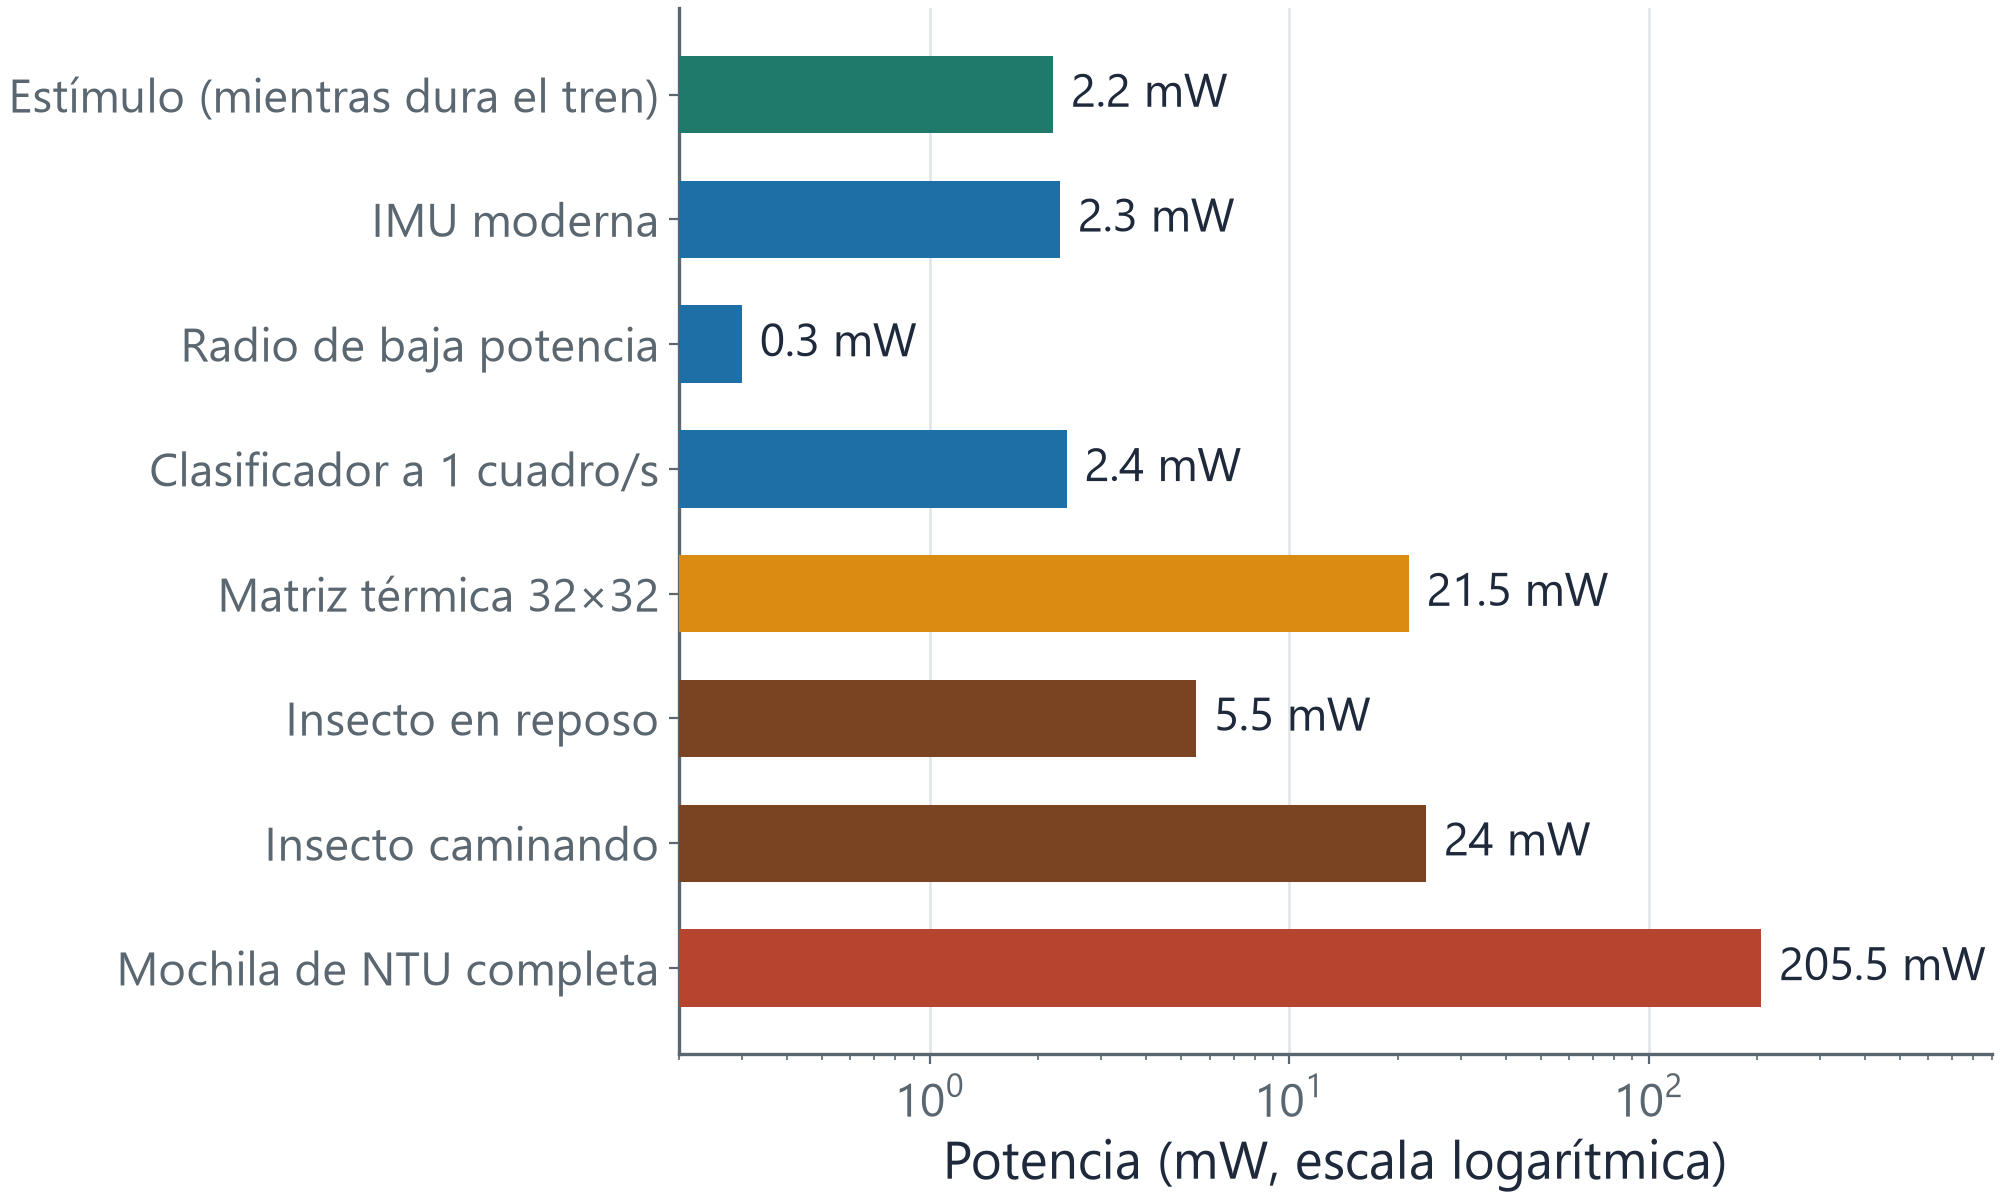
\includegraphics[width=\linewidth]{figs/energia.png}
\caption{Quién gasta qué.}
\end{subfigure}
\caption{Presupuestos de la mochila. La batería y el sensor térmico mandan en la masa; el sensor manda
en la energía. Masas de batería y sensor medidas~\cite{tranngoc2023}; las de los chips son estimadas.}
\label{fig:presupuestos}
\end{figure}

Se adopta la configuración media: matriz térmica, radio de baja potencia, IMU y una batería de
40~mAh, unos 2.9~g. Con el sensor encendido todo el tiempo consume cerca de 30~mW y la
autonomía estimada es
\begin{equation}
t=\frac{0.85\times40~\text{mAh}\times3.7~\text{V}}{30~\text{mW}}\approx4~\text{h},
\end{equation}
que sube a unas 10~h si el sensor trabaja la cuarta parte del tiempo. Como referencia medida,
la mochila de NTU consume 205.5~mW y dura 2.2~h con 120~mAh~\cite{tranngoc2023}.

\textbf{Relación entre carga y capacidad de cómputo.} El cómputo casi no pesa
(tabla~\ref{tab:computo}): una FPGA de 1\,248 LUT cabe en 2~mm$^2$. Lo que el insecto no
puede cargar son baterías grandes ni sensores altos. Por eso conviene gastar lógica, que es
gratis en masa, para ahorrar energía y estímulos.

\begin{table}[H]
\centering\footnotesize
\caption{Qué cómputo cabe en la mochila. Masas estimadas a partir del encapsulado.}
\label{tab:computo}
\rowcolors{2}{SoftGray}{white}
\begin{tabularx}{\textwidth}{@{}>{\bfseries\raggedright\arraybackslash}p{3.7cm} >{\raggedright\arraybackslash}p{2.6cm} >{\raggedright\arraybackslash}p{1.6cm} >{\raggedright\arraybackslash}p{2.2cm} >{\raggedright\arraybackslash}X@{}}
\toprule
\rowcolor{TableHead} Dispositivo & Tamaño & Masa & Reposo & Capacidad \\
\midrule
nRF52840 (radio y procesador)~\cite{nordic} & $3.5\times3.6$~mm & $\approx15$~mg & 0.4~$\mu$A & Cortex-M4, 1~MB; transmite con 6.4~mA \\
iCE40 UltraLite UL1K~\cite{lattice} & $1.4\times1.4$~mm & $\approx2$~mg & 35~$\mu$A & 1\,248 LUT: aloja el núcleo (477) \\
iCE40 UltraPlus UP5K~\cite{lattice} & $2.15\times2.55$~mm & $\approx6$~mg & 75~$\mu$A & 5\,280 LUT, 8 multiplicadores \\
Chip propio en SKY130~\cite{tinytapeout} & $160\times100~\mu$m por módulo & $<1$~mg & Por medir & Unas 1\,000 compuertas por módulo \\
Tarjeta de desarrollo (XIAO, SuperMini) & $21\times18$~mm & 1.5 a 2.5~g & 44~$\mu$A o más & Solo para la maqueta: consume la carga útil \\
\bottomrule
\end{tabularx}
\end{table}

\subsection{M4. La detección}
\label{sec:deteccion}

Un sensor térmico de un solo píxel promedia todo su campo de visión. Si el blanco tiene área
$A$ y está a distancia $d$, solo llena una fracción $f$ del campo, y la lectura es
\begin{equation}
T_{\text{leída}}=T_f+f\,(T_p-T_f),\qquad
f=\min\!\left(1,\ \frac{A}{\pi\,d^2\tan^2(\varphi/2)}\right).
\end{equation}
Con una cara ($A=0.03$~m$^2$), piel a 33~\textdegree C, fondo a 22~\textdegree C y campo de
$\varphi=90$\textdegree, a medio metro la lectura es de 22.4~\textdegree C. Un umbral fijo de
35.5 a 38.5~\textdegree C no se alcanza ni pegado a la persona, porque ese intervalo es de
temperatura central y la piel expuesta está entre 27 y 35~\textdegree C.

Una matriz resuelve el problema, porque cada píxel ve un ángulo pequeño $\theta$ y el blanco
ocupa
\begin{equation}
n=\frac{A}{(d\tan\theta)^2}\quad\text{píxeles}.
\end{equation}
El núcleo cuenta como caliente todo píxel que esté entre 28 y 38~\textdegree C, el criterio de
NTU~\cite{tranngoc2023}, \emph{y además} 2~\textdegree C por encima de la media del cuadro
anterior, para que un ambiente tibio no llene la imagen. Con 2 píxeles empieza a acercarse y
con 8 durante cuatro cuadros seguidos declara la detección (figura~\ref{fig:deteccion}).

\begin{figure}[H]
\centering
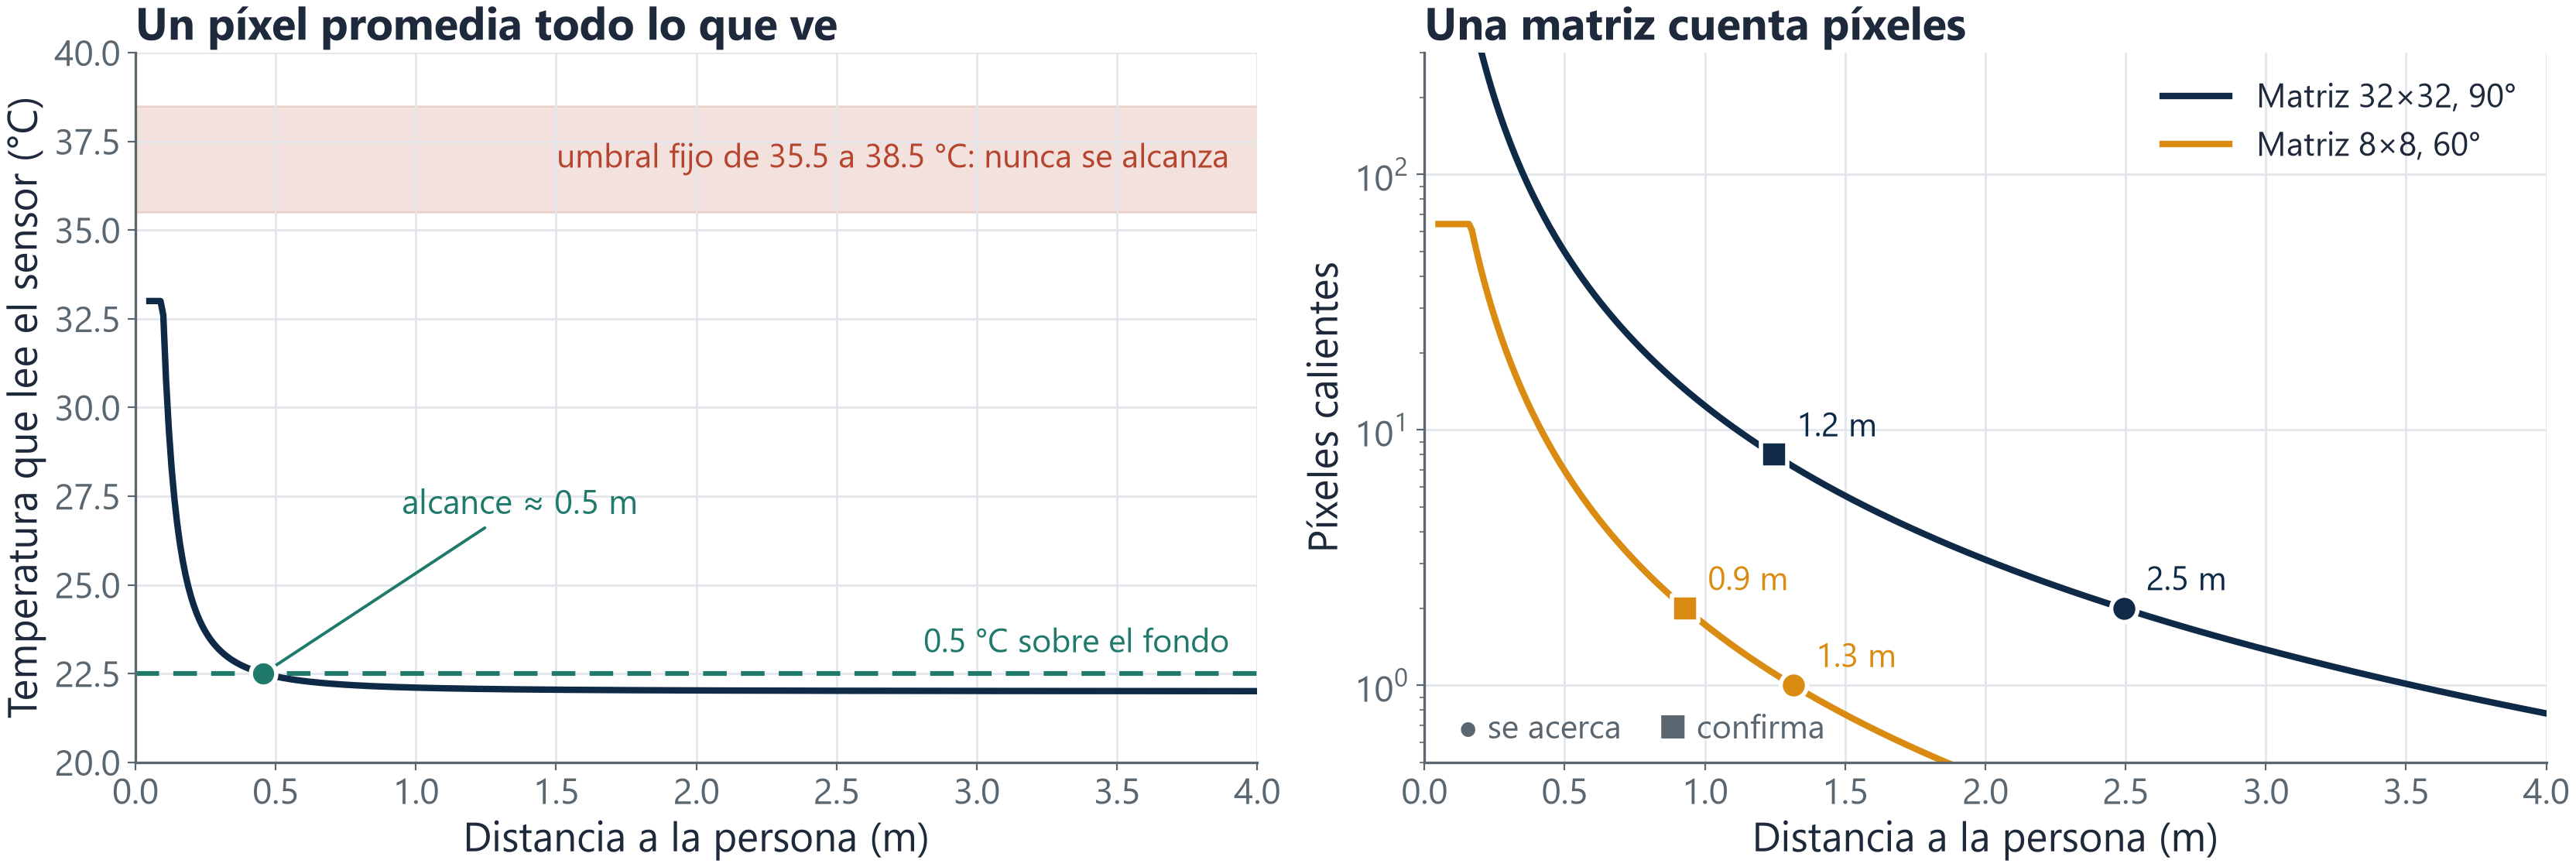
\includegraphics[width=\textwidth]{figs/deteccion_termica.png}
\caption{Izquierda: lectura de un píxel de 90\textdegree{} frente a la distancia. Derecha: píxeles calientes
con dos matrices; el círculo marca dónde empieza el acercamiento y el cuadro dónde se confirma.}
\label{fig:deteccion}
\end{figure}

\begin{table}[H]
\centering\footnotesize
\caption{Sensores térmicos candidatos. Precios de mostrador en México al 9 de noviembre de 2026~\cite{unit}.}
\label{tab:sensores}
\rowcolors{2}{SoftGray}{white}
\begin{tabularx}{\textwidth}{@{}>{\bfseries\raggedright\arraybackslash}p{3.4cm} >{\raggedright\arraybackslash}p{2.0cm} >{\raggedright\arraybackslash}p{1.9cm} >{\raggedright\arraybackslash}p{2.6cm} >{\raggedright\arraybackslash}X@{}}
\toprule
\rowcolor{TableHead} Sensor & Píxeles y campo & Consumo & Alcance (acercar / confirmar) & Precio \\
\midrule
MLX90614 (un punto)~\cite{melexis} & 1; 90\textdegree & Sin verificar & 0.6 / 0.4~m & 189~MXN \\
AMG8833~\cite{panasonic} & $8\times8$; 60\textdegree & 4.5~mA & 1.3 / 0.9~m & 599~MXN \\
MLX90640~\cite{melexis} & $32\times24$; 55\textdegree & $<23$~mA & 4.1 / 2.0~m & 1\,100~MXN \\
Heimann HTPA32x32d~\cite{tranngoc2023} & $32\times32$; 90\textdegree & 6.5~mA & 2.5 / 1.2~m & Sin precio local \\
\bottomrule
\end{tabularx}
\end{table}

\textbf{Límites de la detección térmica.} Si el ambiente pasa de unos 30~\textdegree C, el
contraste con la piel se pierde: en Myanmar el ambiente rondaba los 38~\textdegree C. A esa
temperatura, además, el insecto pasa inmóvil más de la mitad del tiempo~\cite{gracidas2026}
(figura~\ref{fig:ventana}). El CO$_2$ exhalado, que llega a 1.6~\% en un hueco
cerrado~\cite{huo2011}, y el sonido son las señales complementarias; quedan como trabajo
futuro porque los sensores de CO$_2$ pequeños responden en 20 a 60~s.

\begin{figure}[H]
\centering
\begin{subfigure}{0.49\textwidth}
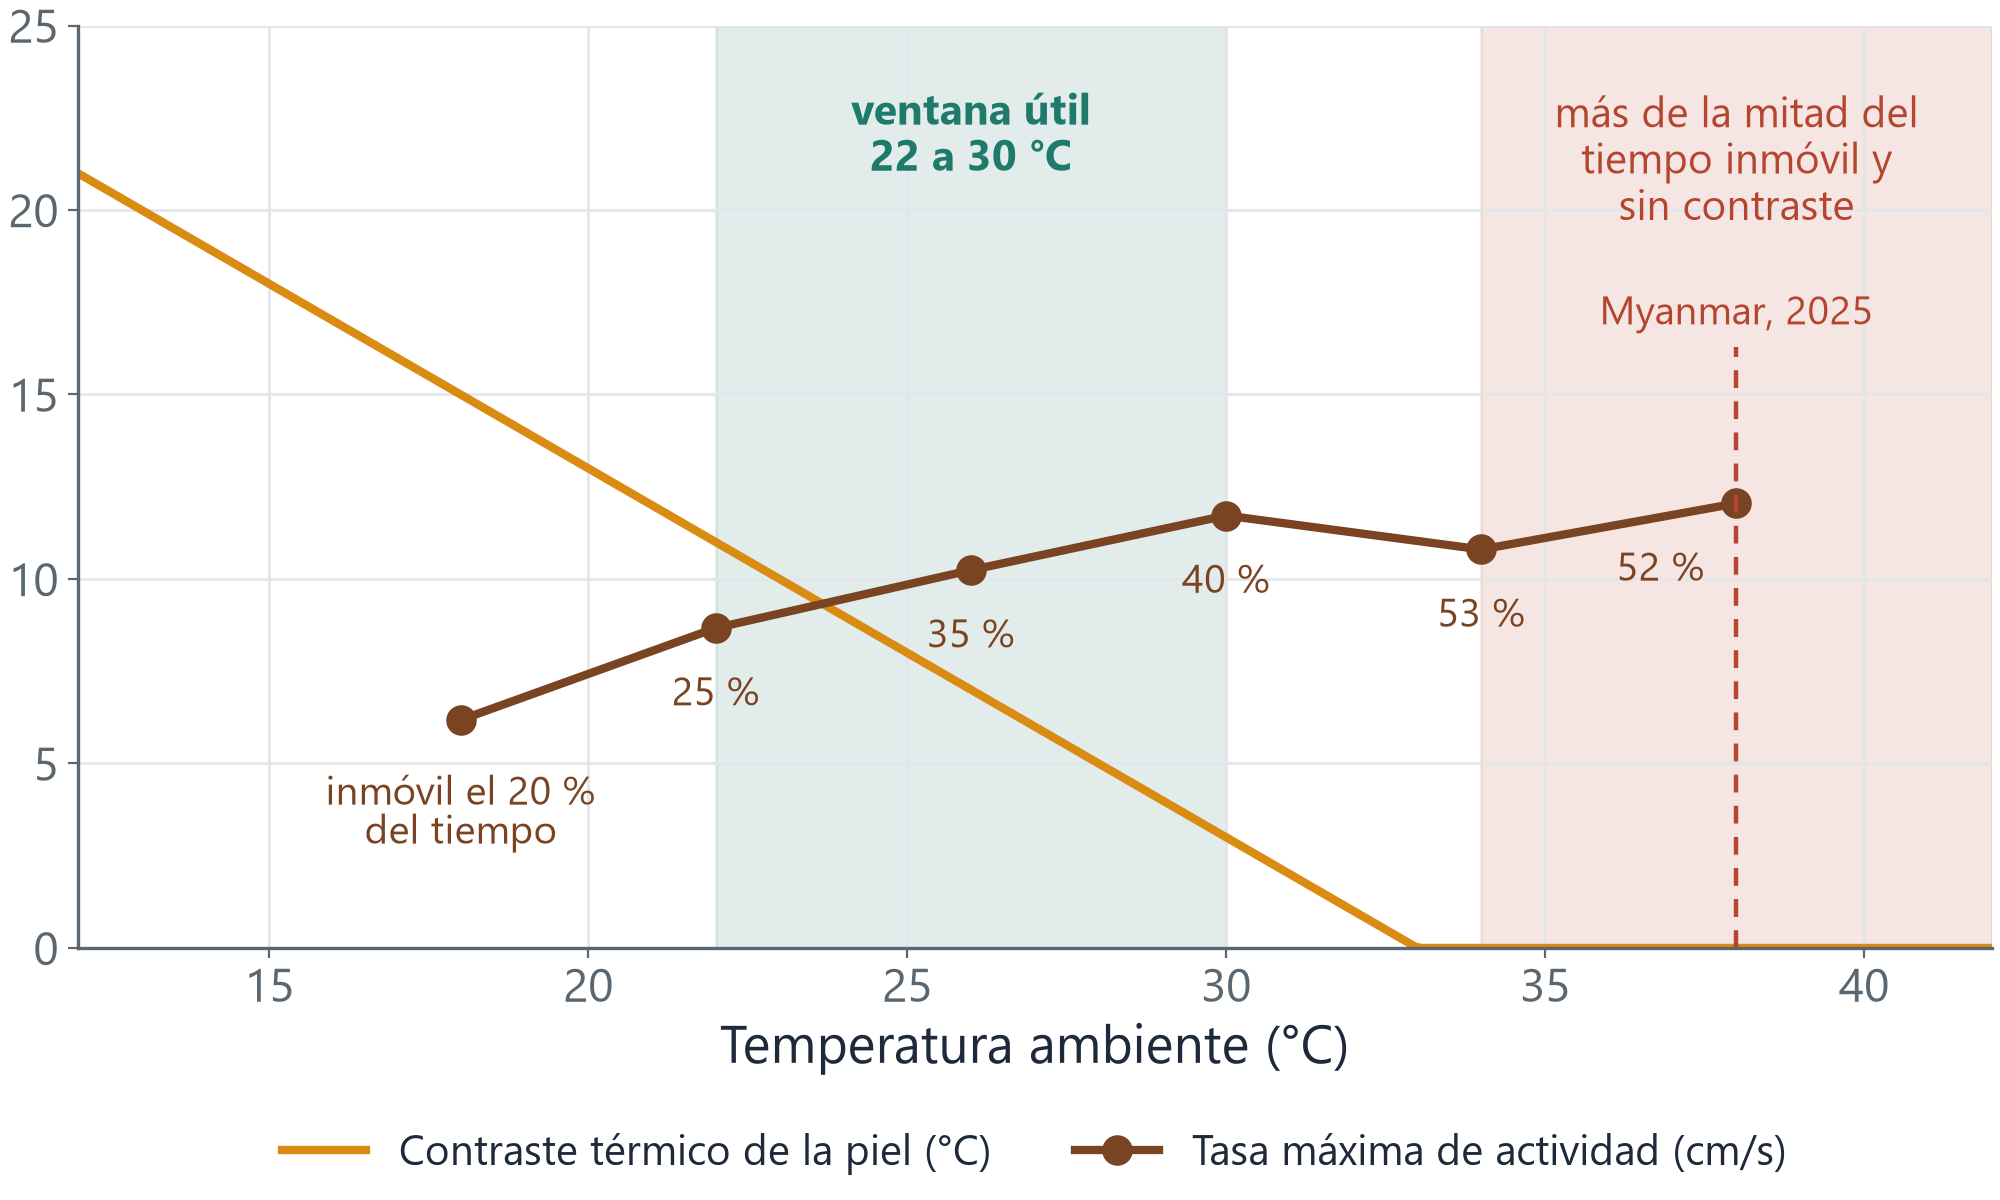
\includegraphics[width=\linewidth]{figs/ventana_operativa.png}
\caption{Ventana de temperatura.}
\label{fig:ventana}
\end{subfigure}\hfill
\begin{subfigure}{0.49\textwidth}
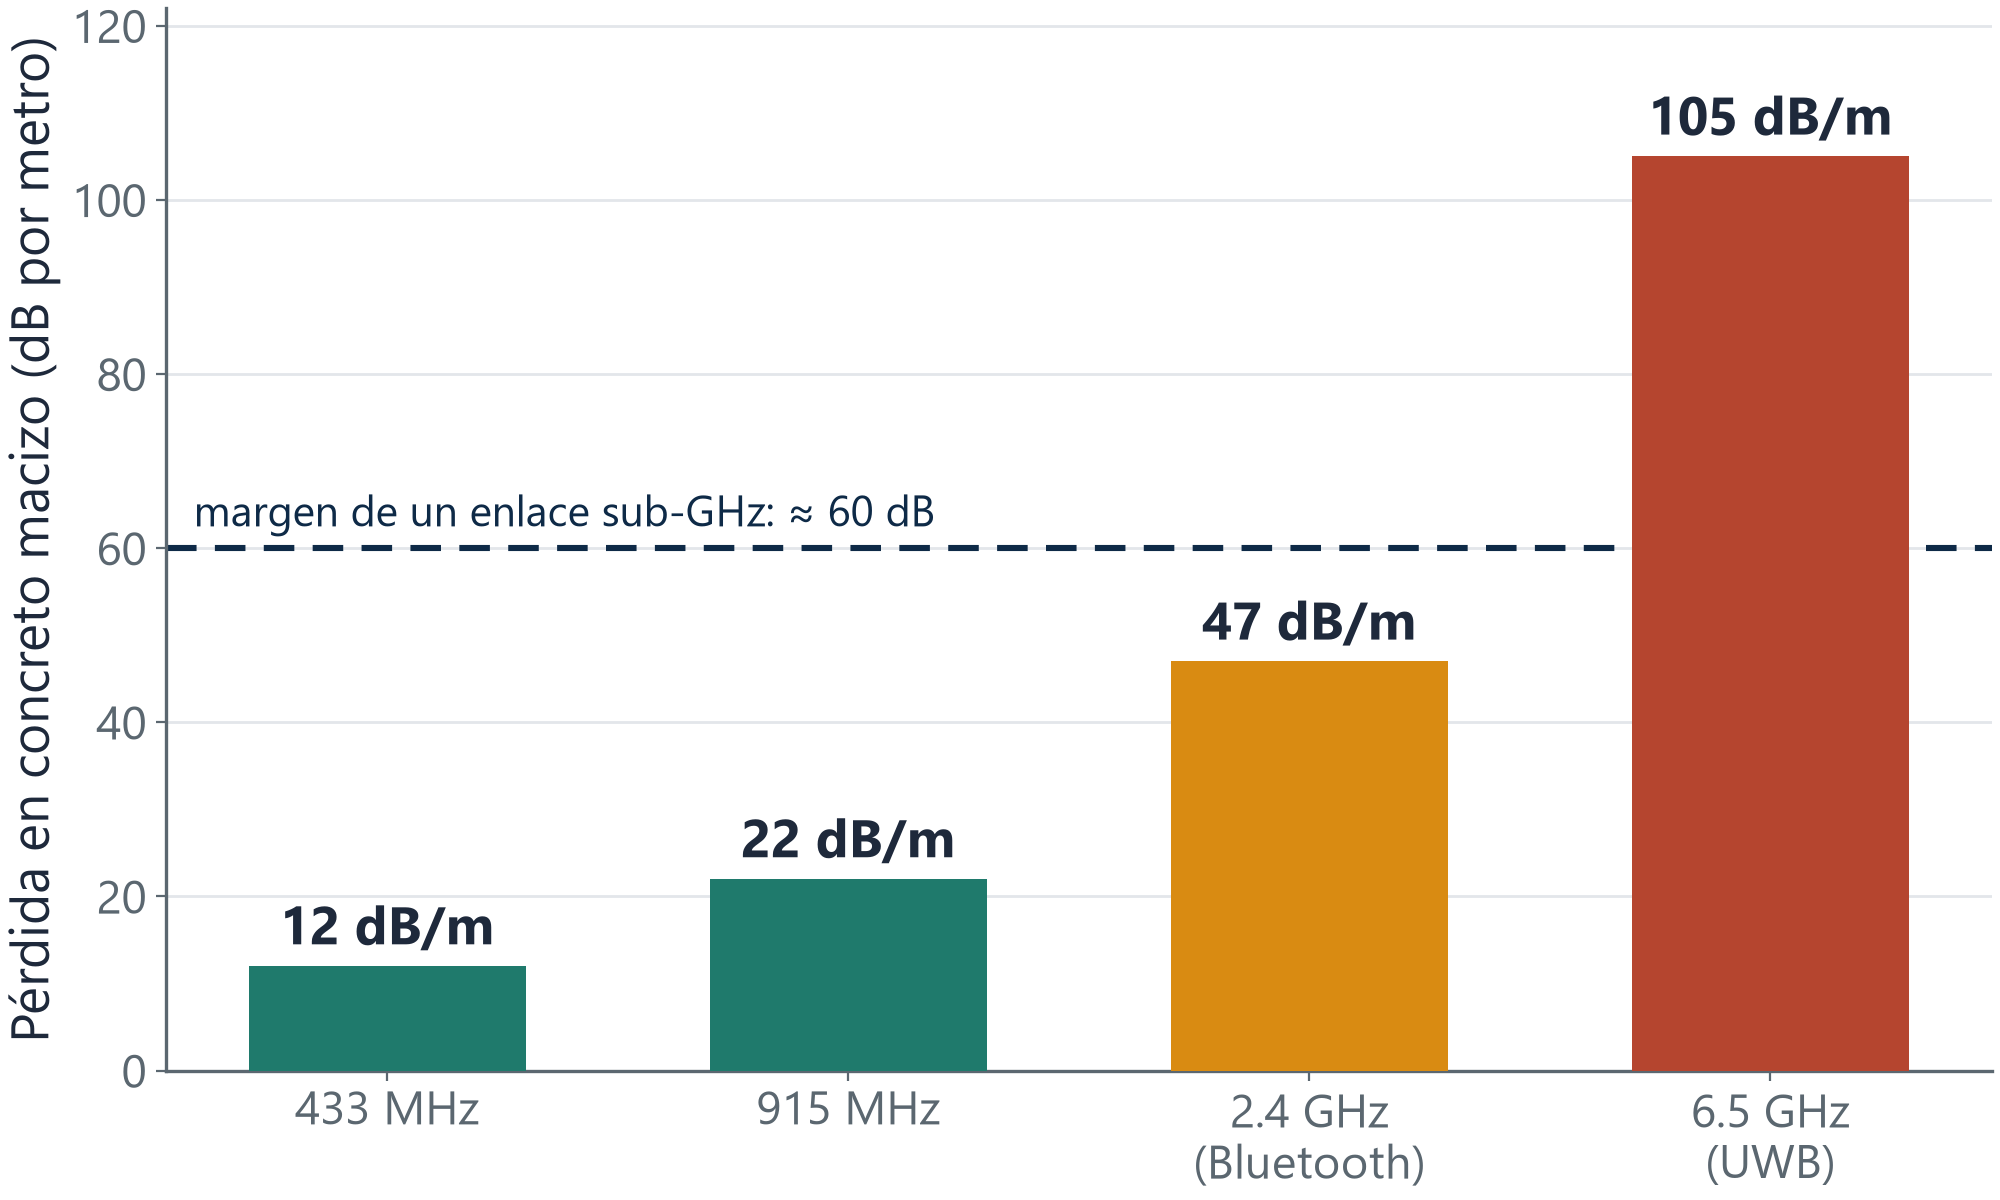
\includegraphics[width=\linewidth]{figs/radio_escombro.png}
\caption{Pérdida de la radio en concreto.}
\label{fig:radio}
\end{subfigure}
\caption{Dos límites prácticos. (a) Contraste térmico disponible y actividad del insecto según la
temperatura~\cite{gracidas2026}. (b) Atenuación calculada con el modelo de la UIT~\cite{itu2040}; las
mediciones de NIST son peores~\cite{stone1997}.}
\end{figure}

\subsection{Localización}

Encontrar a la persona no basta: hay que decirle al rescatista dónde cavar. El método tiene
tres capas, de la más gruesa a la más fina.
\begin{enumerate}
  \item \textbf{Por dónde entró.} Cada mochila tiene un identificador y se libera por un boquete
        conocido. La alerta ya dice en qué zona buscar.
  \item \textbf{Cuánto caminó.} La IMU estima el recorrido contando la actividad de la marcha.
        El error publicado es de 5~\% de la distancia en terreno plano y 10~\% con
        desniveles~\cite{tranngoc2024}: tras 12~m, entre 0.6 y 1.2~m (figura~\ref{fig:localizacion}).
  \item \textbf{El último medio metro.} Al confirmar, la mochila deja de estimular, el insecto se queda
        donde está y emite una baliza de radio y de luz cada 5~s. El tamaño de la mancha da además
        la distancia a la persona: $d\approx\sqrt{A/n}\,/\tan\theta$.
\end{enumerate}
La radio debe ser de menos de 1~GHz. El concreto atenúa unos 22~dB por metro a 915~MHz y 47~dB
a 2.4~GHz~\cite{itu2040}, y el único robot inalámbrico del World Trade Center se perdió a unos
10~m de la entrada~\cite{murphy2004}. Un relevo en el boquete acorta el enlace.

\begin{figure}[H]
\centering
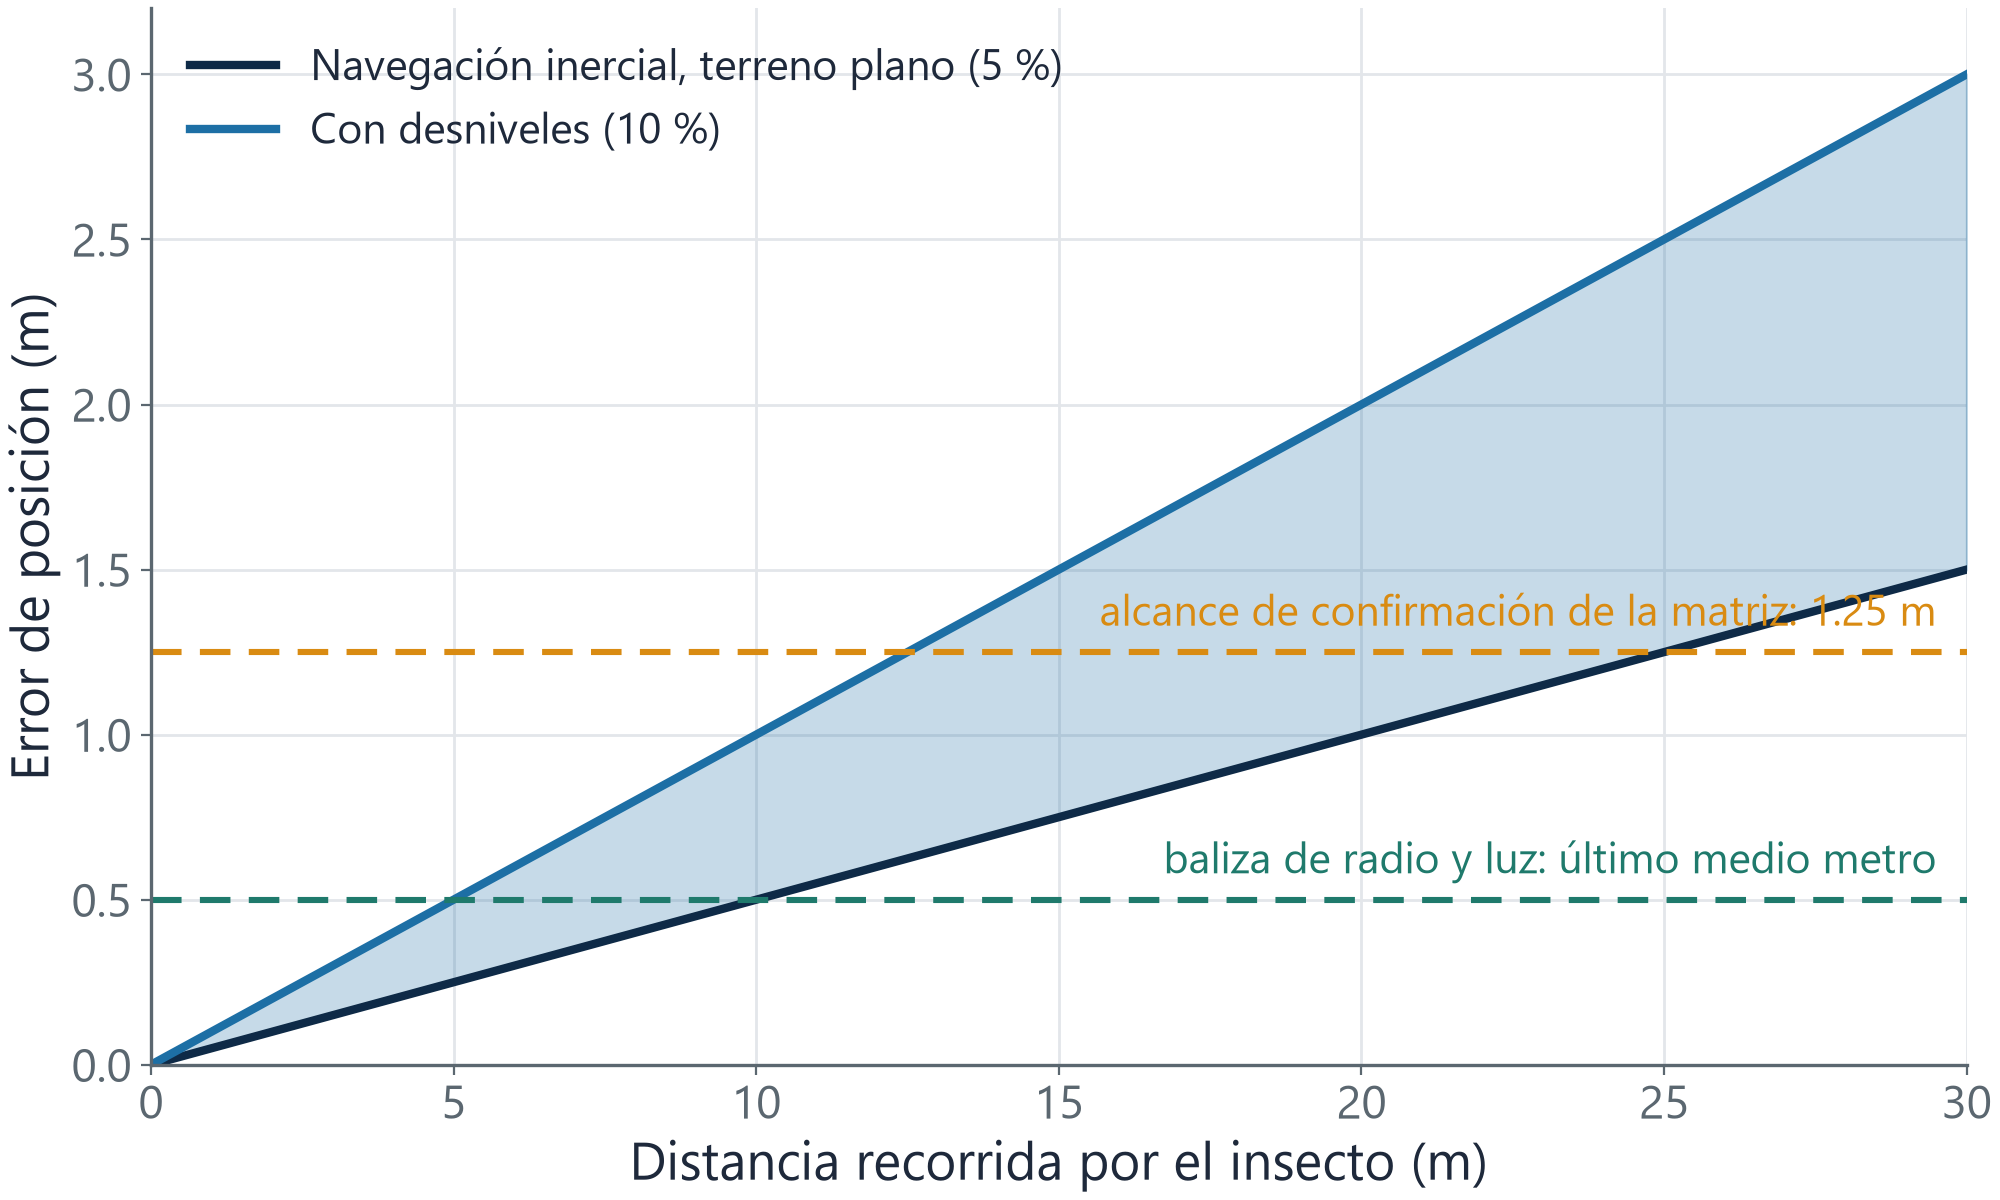
\includegraphics[width=0.62\textwidth]{figs/localizacion.png}
\caption{Error de posición por navegación inercial frente a la distancia recorrida.}
\label{fig:localizacion}
\end{figure}

\subsection{M5. La misión}

La misión se simula con agentes. Cada agente camina con el modelo de M1, obedece estímulos
con el modelo de M2 y detecta con el de M4, dentro de un colapso sintético de $8\times6$~m
hecho de losas y escombro con huecos conectados (figura~\ref{fig:mapa}). Se comparan cuatro
políticas: pasiva (sin estímulos), antipausa, estocástica (antipausa más giros al azar) y guiada
(además se acerca a la mancha de calor). Como referencia analítica, la teoría de búsqueda da
para una búsqueda al azar~\cite{frost2001}
\begin{equation}
P_d=1-e^{-C},\qquad C=\frac{W\,v\,t\,N}{A_h},
\end{equation}
con ancho de barrido $W$, velocidad $v$, tiempo $t$, $N$ insectos y área de huecos $A_h$.

\begin{table}[H]
\centering\footnotesize
\caption{Parámetros principales de la simulación. F: publicado; D: decisión de diseño; S: supuesto que
se explora en el análisis de sensibilidad.}
\label{tab:parametros}
\rowcolors{2}{SoftGray}{white}
\begin{tabularx}{\textwidth}{@{}>{\raggedright\arraybackslash}X >{\raggedright\arraybackslash}p{3.0cm} c >{\raggedright\arraybackslash}p{4.0cm}@{}}
\toprule
\rowcolor{TableHead} \textbf{Parámetro} & \textbf{Valor} & \textbf{Origen} & \textbf{Fuente} \\
\midrule
Velocidad natural & $1.94\pm0.29$~cm/s & F & \cite{dirafzoon2017} \\
Tramo recto, media & 17.6~cm & F & \cite{dirafzoon2017} \\
Probabilidad de pausa por tramo & 0.211 & F & \cite{dirafzoon2017} \\
Duración de la pausa & $36.8\pm24.1$~s & F & \cite{dirafzoon2017} \\
Probabilidad de soltar la pared & 0.005 & F & \cite{dirafzoon2017} \\
Probabilidad de obedecer un estímulo & 0.78 & F & \cite{lin2023} \\
Giro por estímulo & $52\pm23$\textdegree & F & \cite{lin2023,lin2025,ma2023} \\
Marcha tras un estímulo de avance & 5~cm/s durante 4~s & F & \cite{tranngoc2024,erickson2015} \\
Habituación por estímulo, $\alpha$ & 0.01 (0.09 unipolar) & F & \cite{erickson2015,ma2023} \\
Recuperación, $\tau$ & 600~s & F & \cite{sanchez2015} \\
Espera antes de reactivar & 15~s, se duplica hasta $\times8$ & D & --- \\
Tiempo mínimo entre estímulos & 10~s & D & como~\cite{ma2023} \\
Giros al azar & uno cada 51~s en promedio & D & --- \\
Presupuesto de estímulos & 12 acumulados; se vacía en 600~s & D & --- \\
Píxeles para acercar y para confirmar & 2 y 8, cuatro cuadros & D & \cite{tranngoc2024} \\
Área de piel a la vista & 0.03~m$^2$ & S & --- \\
Dobla esquinas pegado a la pared & 0.80 & S & --- \\
Insectos perdidos por hora & 0 & S & --- \\
\bottomrule
\end{tabularx}
\end{table}
